\section{Analyse des résultats}
La figure \ref{fig:ResultatsChampsSigma} donnent une illustration des champs des contraintes pour différentes discrétisations. La table \ref{table:objectif} reprend différentes valeurs de l'objectif obtenues pour pour différentes discrétisations et différentes valeurs de $k$. La valeur optimale croit bien avec le nombre de triangles, comme prédit par la théorie (voir section Modélisation). Celle-ci est bien entendue croissante (linéairement) avec $k$. Cependant la formes des champs de contraintes restent similaire pour différentes valeurs de $k$, comme nous le montre la figure \ref{fig:ResultatsChampsSigma}. On peut donc, sans connaître la valeur $k$ du matériaux, représenter l'allure des champs de contraintes. On peut aussi représenter le champs des valeurs de la contrainte de plasticité de von Mises, cf. figures \ref{fig:Tresca} et \ref{fig:TrescaUp}; et prédire ainsi les premières zones qui devraient présenter des déformations plastiques si la charge était augmentée.

\begin{table}[h!]
\centering
\begin{tabular}{c|cccc}
\textbf{Discrétisation} & $N=4$ & $N=8$ & $N=12$ & $N=16$\\
\textbf{Valeur de l'objectif} ($k=1$) & 1.3483 & 1.379409 & 1.3866 & 1.393687 \\
\textbf{Valeur de l'objectif} ($k=2$) & 2.6967 & 2.7588 & 2.7778 & 2.7880\\
\textbf{Valeur de l'objectif} ($k=4$) & 5.3934 & 5.5180 & 5.5563 & 5.5769
\end{tabular}
\caption{Valeur de l'objectif.}
\label{table:objectif}
\end{table} 

\begin{figure}[h!]
  \centering
  \begin{subfigure}[b]{0.32\textwidth}
  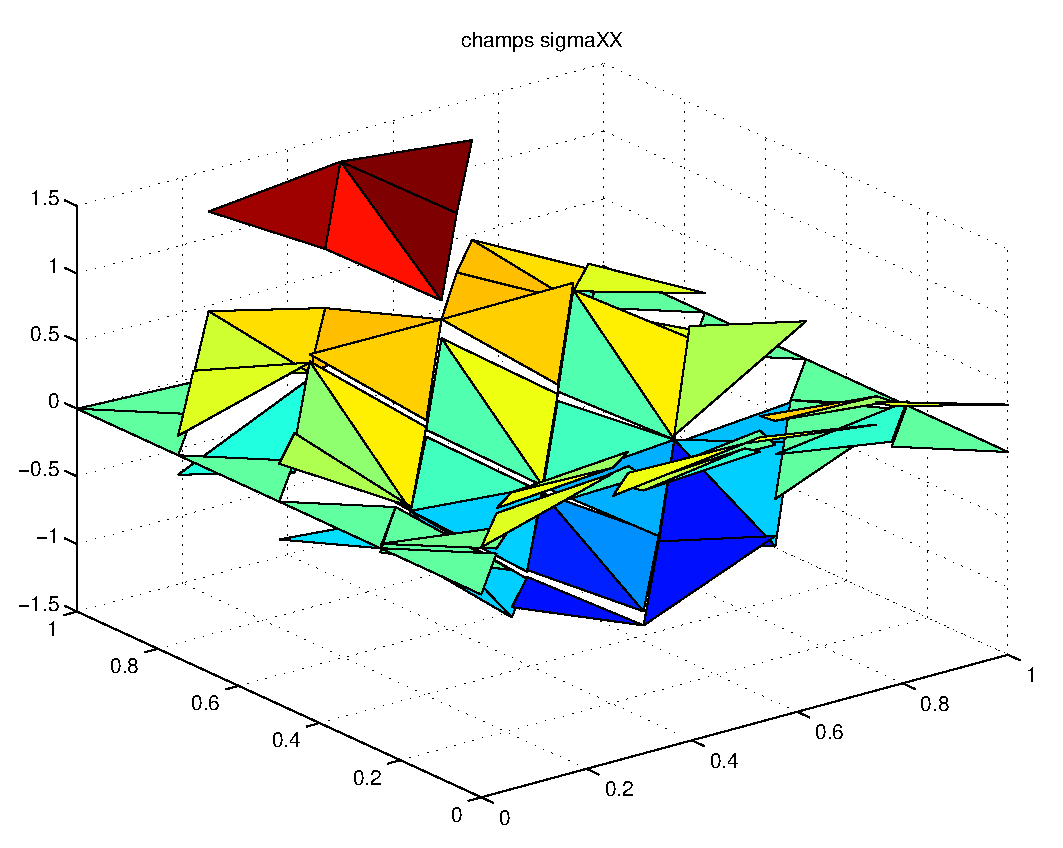
\includegraphics[width=\textwidth]{images/sigmaxxN4.eps}
  \caption{Champs $\sigma_{xx}$ pour $N=4$, $k=1$}
  \end{subfigure}%
  ~
  \begin{subfigure}[b]{0.32\textwidth}
  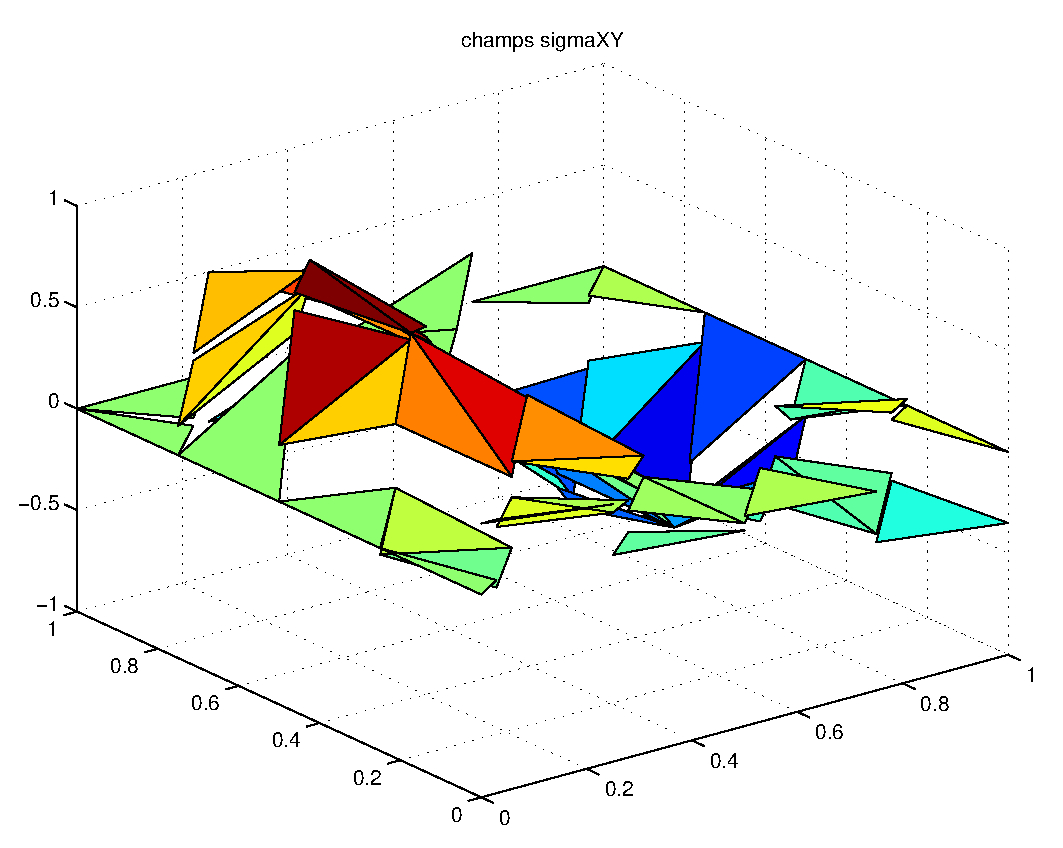
\includegraphics[width=\textwidth]{images/sigmaxyN4.eps}
  \caption{Champs $\sigma_{xy}$ pour $N=4$, $k=1$}
  \end{subfigure}
  ~
  \begin{subfigure}[b]{0.32\textwidth}
  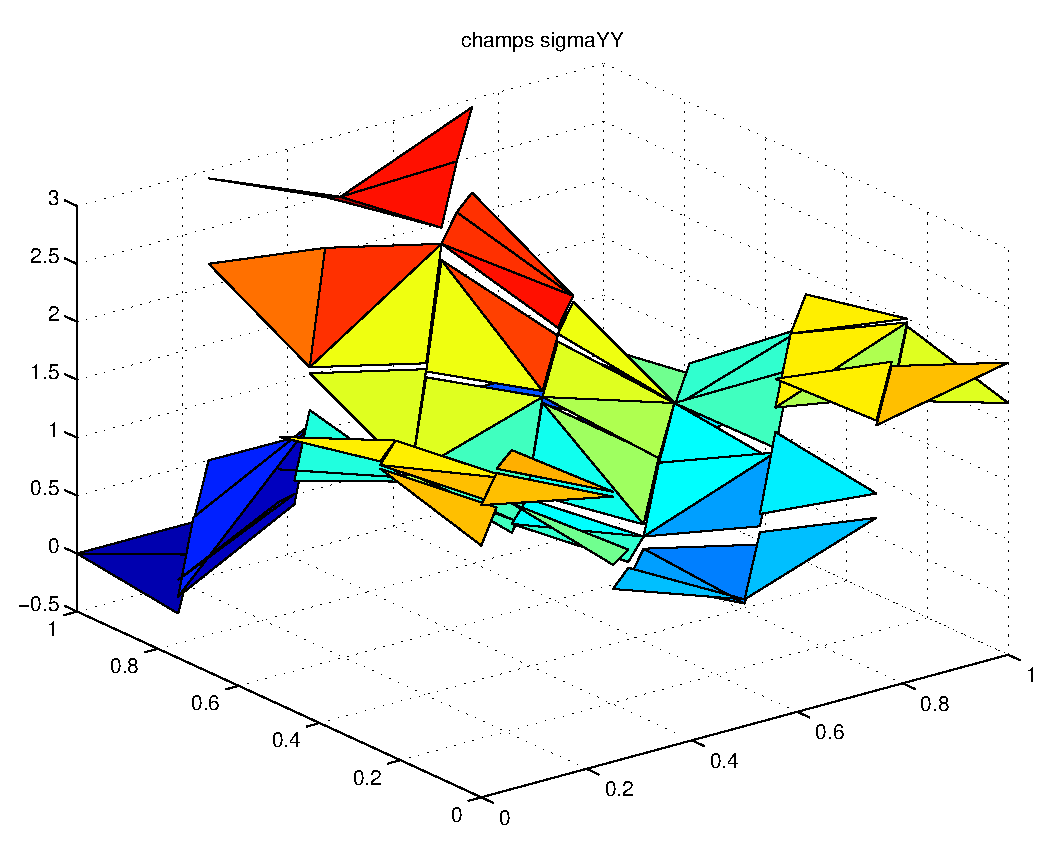
\includegraphics[width=\textwidth]{images/sigmayyN4.eps}
  \caption{Champs $\sigma_{yy}$ pour $N=4$, $k=1$}
  \end{subfigure}
  \begin{subfigure}[b]{0.32\textwidth}
  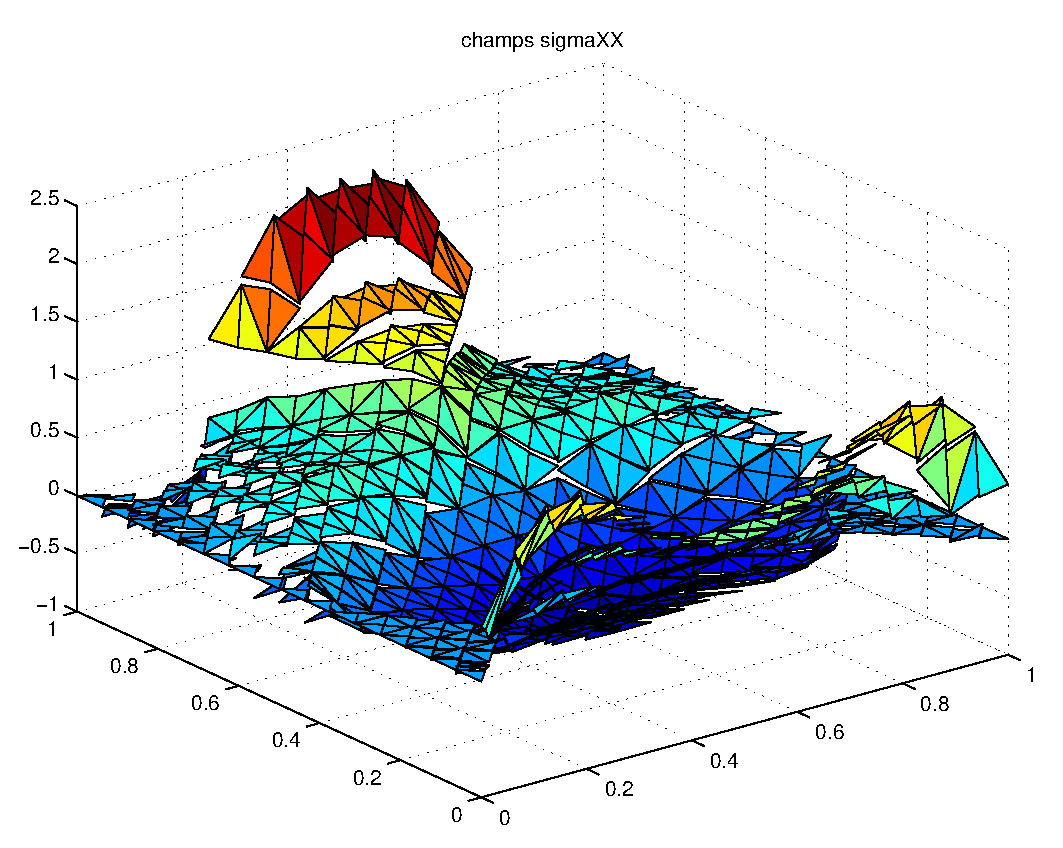
\includegraphics[width=\textwidth]{images/sigmaxxN32.eps}
  \caption{Champs $\sigma_{xx}$ pour $N=16$, $k=1$}
  \end{subfigure}
  ~
  \begin{subfigure}[b]{0.32\textwidth}
  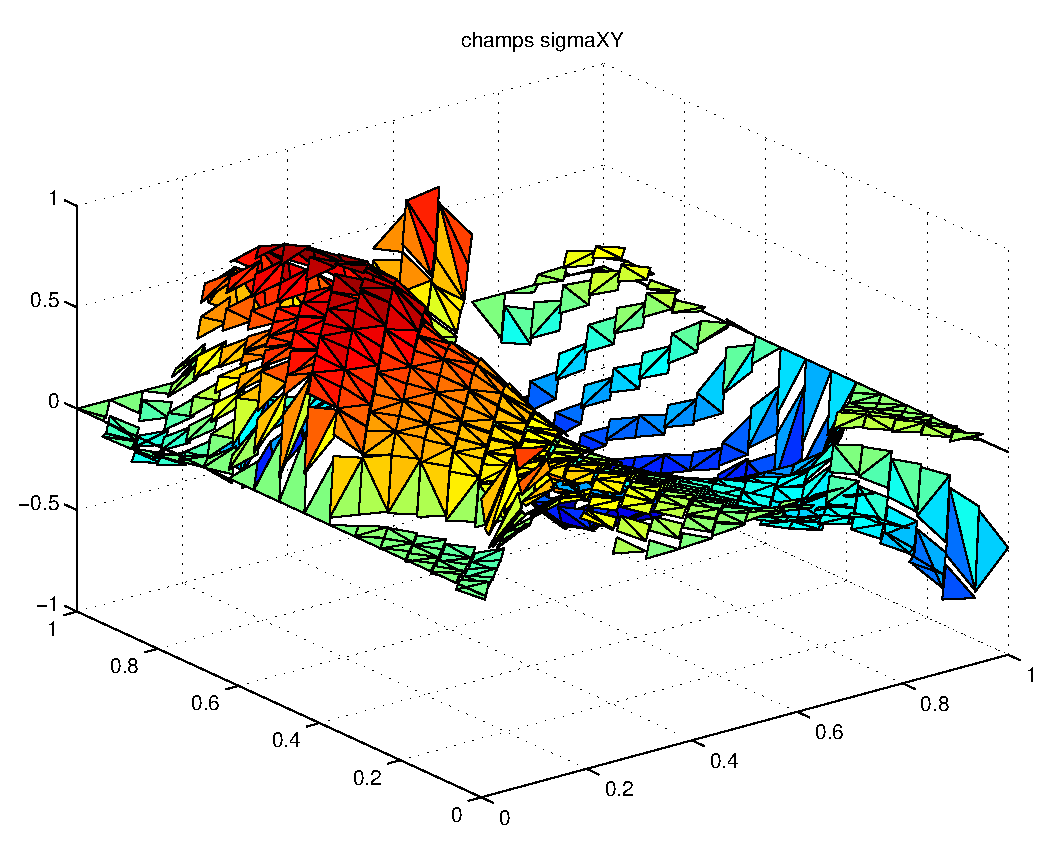
\includegraphics[width=\textwidth]{images/sigmaxyN32.eps}
  \caption{Champs $\sigma_{xy}$ pour $N=16$, $k=1$}
  \end{subfigure}
  ~
  \begin{subfigure}[b]{0.32\textwidth}
  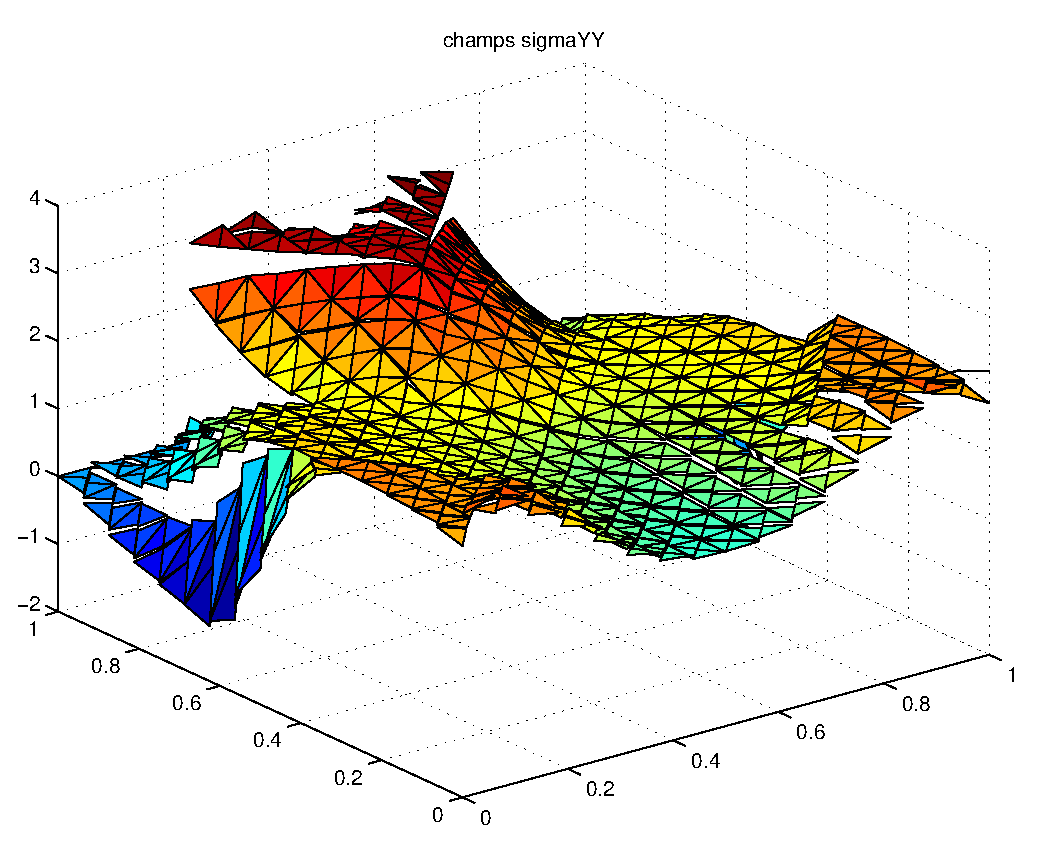
\includegraphics[width=\textwidth]{images/sigmayyN32.eps}
  \caption{Champs $\sigma_{yy}$ pour $N=16$, $k=1$}
  \end{subfigure}
  \begin{subfigure}[b]{0.32\textwidth}
  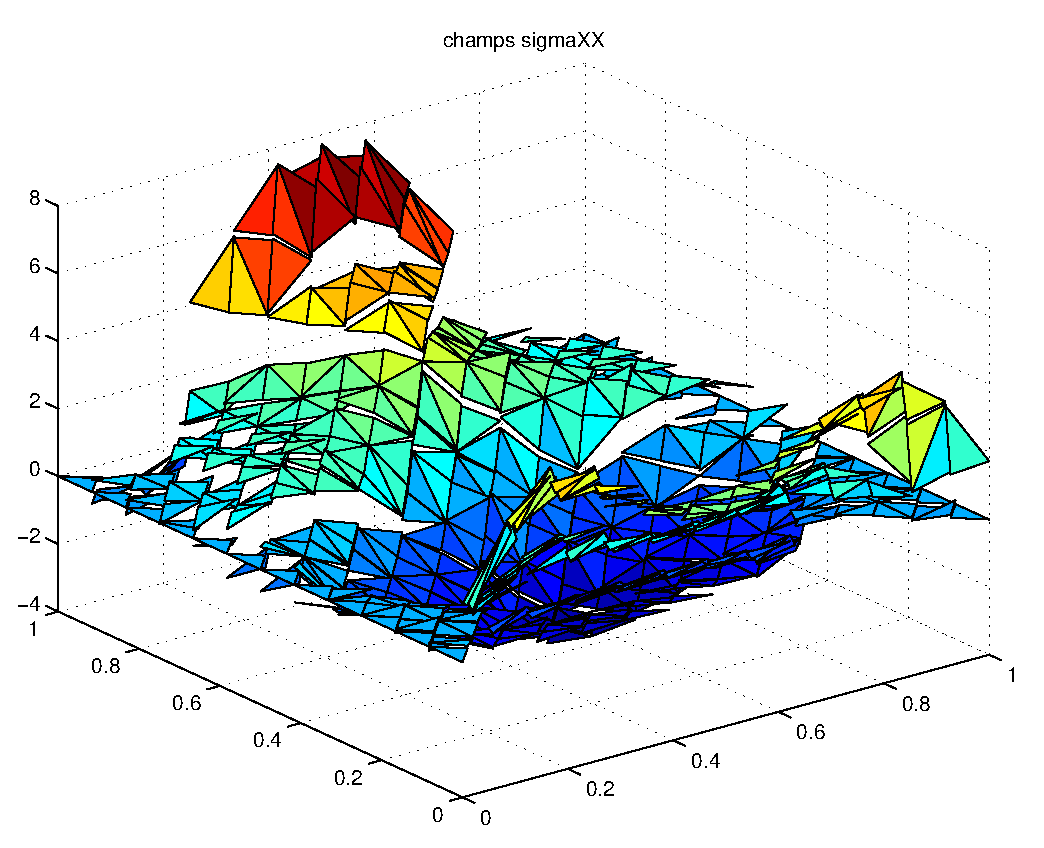
\includegraphics[width=\textwidth]{images/sigmaxxk4.eps}
  \caption{Champs $\sigma_{xx}$ pour $N=12$, $k=4$}
  \end{subfigure}
  ~
  \begin{subfigure}[b]{0.32\textwidth}
  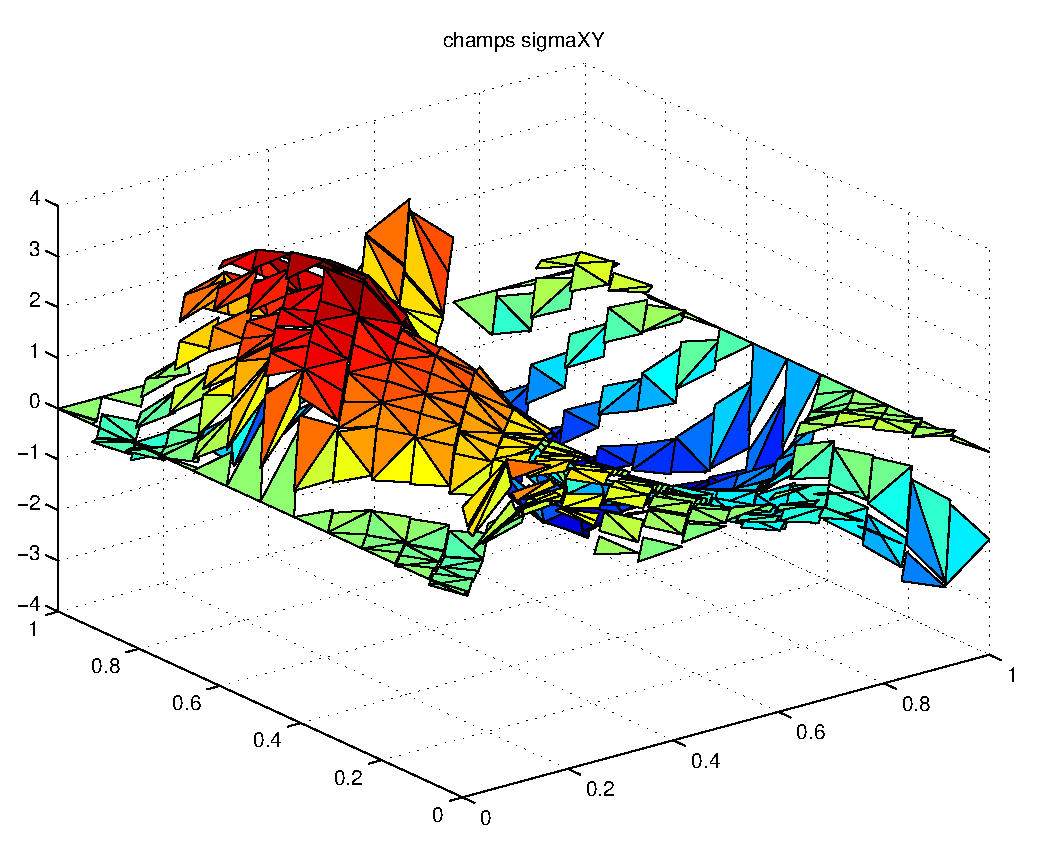
\includegraphics[width=\textwidth]{images/sigmaxyk4.eps}
  \caption{Champs $\sigma_{xy}$ pour $N=12$, $k=4$}
  \end{subfigure}
  ~
  \begin{subfigure}[b]{0.32\textwidth}
  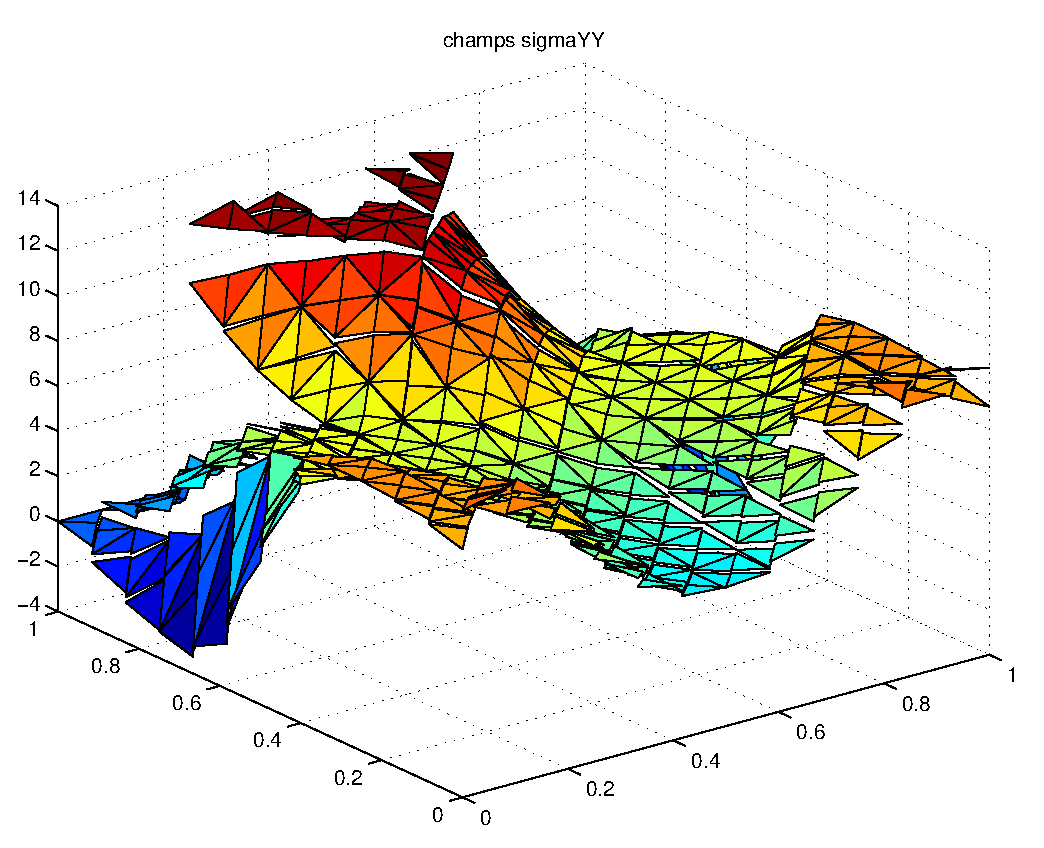
\includegraphics[width=\textwidth]{images/sigmayyk4.eps}
  \caption{Champs $\sigma_{yy}$ pour $N=12$, $k=4$}
  \end{subfigure}
  \begin{subfigure}[b]{0.32\textwidth}
  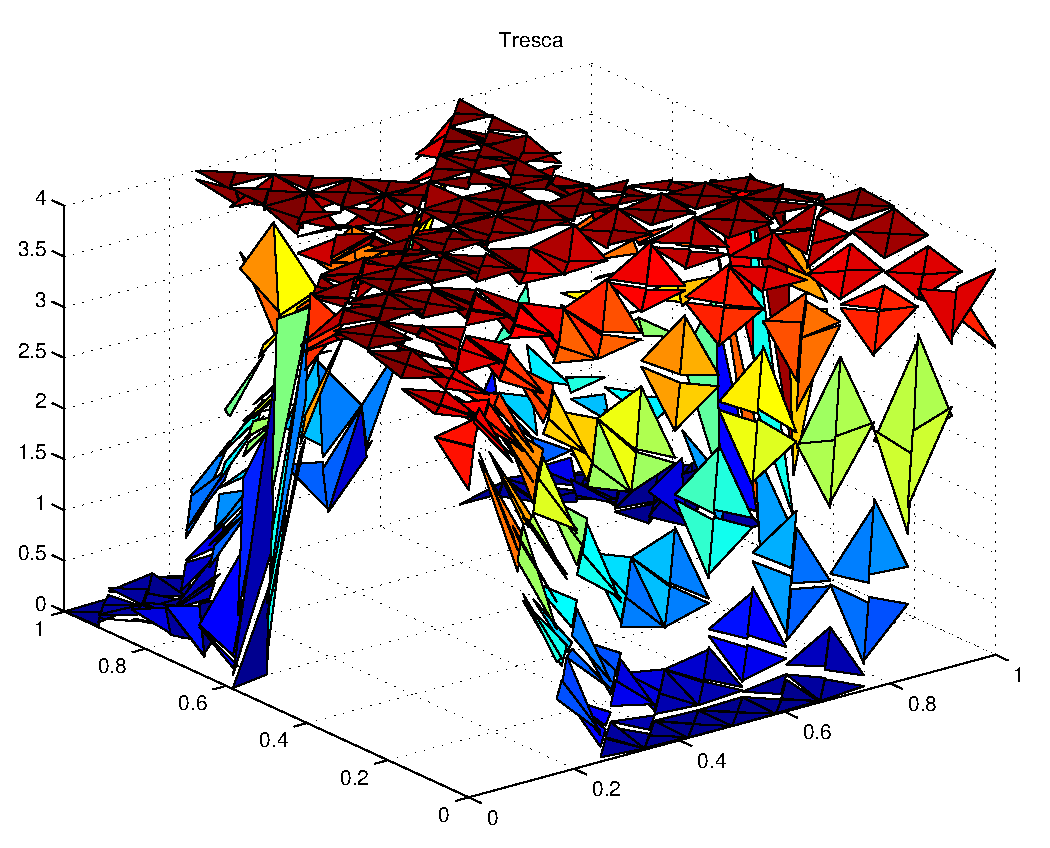
\includegraphics[width=\textwidth]{images/Tresca.eps}
  \caption{Champs des contraintes de Tresca, $N=12$, $k=1$}
  \label{fig:Tresca}
  \end{subfigure}
  ~
  \begin{subfigure}[b]{0.32\textwidth}
  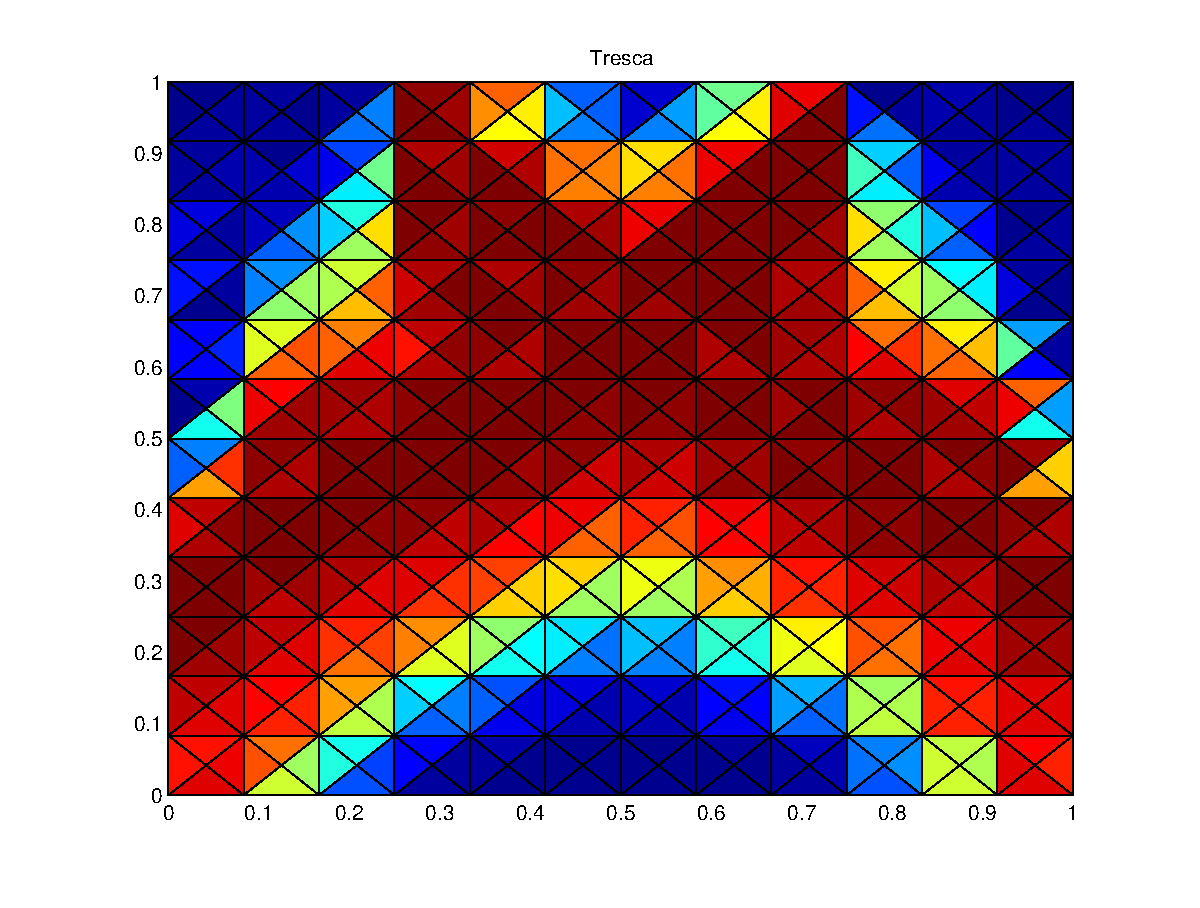
\includegraphics[width=\textwidth]{images/TrescaUp.eps}
  \caption{Champs des contraintes de Tresca, $N=12$, $k=1$ (vu du haut)}
    \label{fig:TrescaUp}
  \end{subfigure}
  ~
  \begin{subfigure}[b]{0.32\textwidth}
  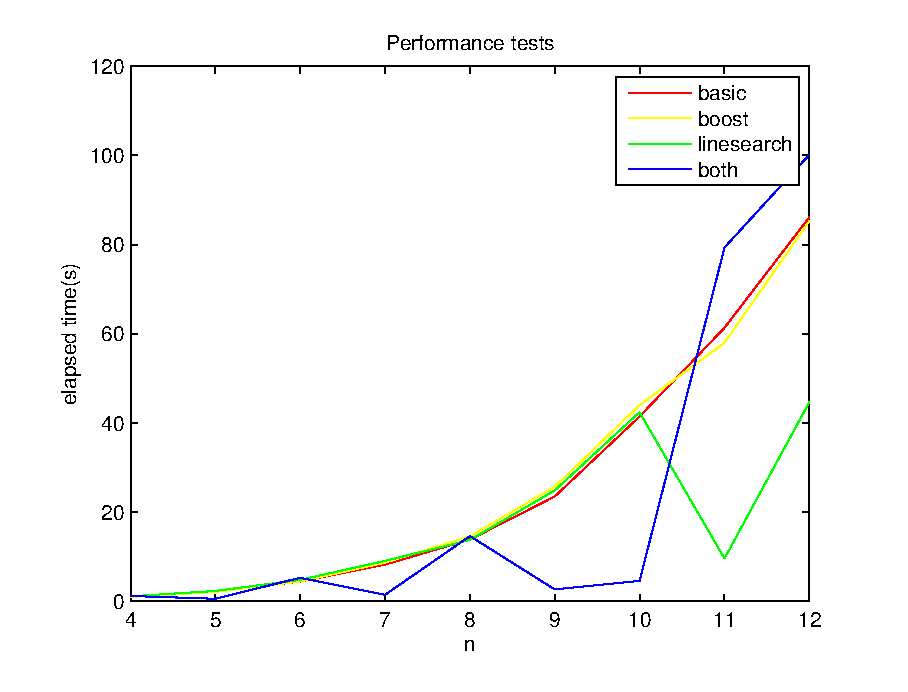
\includegraphics[width=6cm]{images/speedimp.eps}
\caption{Evolution des temps de calcul pour la méthode et ses "améliorations"\label{fig:speedimp}}
  \end{subfigure}
  \caption{}
  \label{fig:ResultatsChampsSigma}
\end{figure}

\subsection{Complexité et performances}
Nous utilisons les paramètres suivant : $\tau = 0.25$, $\sigma_{initial} = 0.1$, $\epsilon = 10^{-4}$, $\nu = \frac{nbVariables}{3}$. Comme les contraintes de Tresca sont des contraintes quadratiques, on a $\nu=1$ pour une contrainte. Or ici on a autant de contraintes que de points c'est-à-dire $\frac{nbVariables}{3}$. La valeur du $\epsilon$ est choisie en fonction de la précision voulue. Notons que $\mu_{final} = \frac{\epsilon}{\sqrt{\nu} + \tau \epsilon}$ détermine le nombre d'itérations barrières. Si $\sigma$ est constant, on a alors, pour nos paramètres, 5 itérations barrières en partant de $\mu_0=1$. 

Rappelons que la complexité de pire cas d'une méthode à pas longs  $\mathcal{O}(\nu log(\frac{1}{\epsilon})$. Bien que cette complexité de pire cas soit supérieure à la complexité de pire cas d'une méthode à pas courts, donnée par $\mathcal{O}(\sqrt{\nu} \log(\frac{1}{\epsilon}))$, elle est en pratique rarement atteinte. En effet, contrairement à la méthode à pas court qui prédit exactement le nombre de Newton-step à exécuter, la méthode à pas long laisse des "latitudes" d'évolution sur le nombre de Newton-step exécuté par itération barrière. A titre d'exemple, pour notre méthode à pas long sans améliorations, le nombre de pas de Newton pour nos paramètres et $N=4$ est de l'ordre de 100, alors que la borne $mathcal{O}(\nu log(\frac{1}{\epsilon}) = 1768$ soit 17 fois plus.


On peut essayer d'améliorer notre méthode et on obtient les résultats de la figure \ref{fig:speedimp}.

Nous avons introduit deux améliorations sous la forme d'heuristiques : 
\begin{itemize}
\item Recherche en ligne : au lieu de proposer un pas de Newton multiplié par $\frac{1}{1+\delta}$ lorsque $\delta>1$, on essaie de trouver la longueur de pas maximale telle que l'itéré reste admissible.
\item $\sigma$ adaptatif : Cette heuristique adapte simplement la valeur de $\sigma$. Intuitivement, si l'on utilise un $\sigma$ plus petit le nombre de pas de Newton nécessaire par étape sera diminué. On diminue donc $\sigma$ quand le nombre de pas de Newton à l'étape précédente sera trop important, et on le diminuera quand il sera petit.
\end{itemize}

